\chapter{Visualisation expérimental d'un mode localisé}
Comme vu précédemment, un défaut dans le réseau provoque un mode localisé. L'objectif est ici de mettre en évidence ce phénomène de manière expérimentale.\\


Un mode localisé dans un tel réseau est à la fois difficile à générer et à observer, expérimentalement comme numériquement. La fréquence de résonance du défaut doit se trouver sur le bord intérieur d'une bande interdite afin de pouvoir la visualiser sur les coefficients de transmission et réflexion. En effet, la propagation de l'onde dans le réseau se fait sur une longueur réduite : la bande interdite rend la décroissance de l'onde exponentielle. Par conséquent, la fréquence de résonance du défaut et la position du défaut par rapport à la source sont cruciales. De plus, une fois le mode généré, il ne peut être observé que très localement et si le réseau est trop grand, il n'est alors pas visible sur les coefficients de transmission et de réflexion qui sont issues de mesures à l'entrée et la sortie du réseau.


\section{Protocole expérimental}
Le banc de mesure utilisé est constitué d'un tuyau perforé de 60 trous sur lesquels peuvent être fixés soit des résonateurs de longueurs de cavité variables (les dimensions sont présentes en annexe), soit des bouchons (cf figure~\ref{photo_manip}. La source utilisée est celle du capteur d'impédance (piézoélectrique) : celui-ci est fixé à une des extrémités du réseau et est relié à une carte d'acquisition piloté par le logiciel spécialisé du CTTM\footnote{Centre de Transfert de Technologie du Mans}. Ce capteur dispose de 2 microphones et permet donc de calculer directement le coefficient de réflexion du réseau. Afin de pouvoir calculer le coefficient de transmission, un autre microphone (\textcolor{red}{reference mic + ampli}) est ajouté à l'autre extrémité du réseau, $10~cm$ après le dernier résonateur.


\textbf{mode }

\todo{photo manip}
\begin{figure}
	\centering
	\includegraphics[scale=0.5]{images_chp3/dscn0123.png}
	\caption{Photo du banc de mesure utilisé.}
\end{figure}

Les mesures de pression dans le guide sont faites par déplacement manuel d'un microphone (\textcolor{red}{reference}) directement placé à l'intérieur du réseau.

\todo{citer une annexe sur la démo du coefficient de transmission et mettre la bonne annexe sur les dims des resonateurs}



\bigskip

A l'autre extrémité du réseau se trouve une sortie anéchoïque préalablement réglée afin que le coefficient de réflexion au bout du réseau soit le plus faible possible. Le coefficient de réflexion du guide sans les résonateurs est en dessous de 8\% pour la bande de fréquence d'intérêt (cf annexe \ref{term_anecho}).


\section{Mesure du coefficient de réflexion et de transmission du réseau}
On s'intéresse tout d'abord à la mesure du coefficient de réflexion et de transmission dans le réseau. Le but est de chercher la fréquence précise à laquelle le mode de défaut a lieu afin de pouvoir par la suite l'observer expérimentalement. Pour cela, on ne prend que 5 résonateurs (avec un défaut sur le troisième) afin que le mode localisé puisse s'étaler sur les bords du réseau et qu'il soit ainsi visible sur les coefficients de réflexion et de transmission. Les résonateurs ont une longueur de cavité de $16~cm$ et le défaut de $8~cm$. Les courbes figure ~\ref{ref1} et ~\ref{trans1} correspondent aux coefficients de réflexion et de transmission pour cette configuration.

\begin{figure}[!h]
\centering
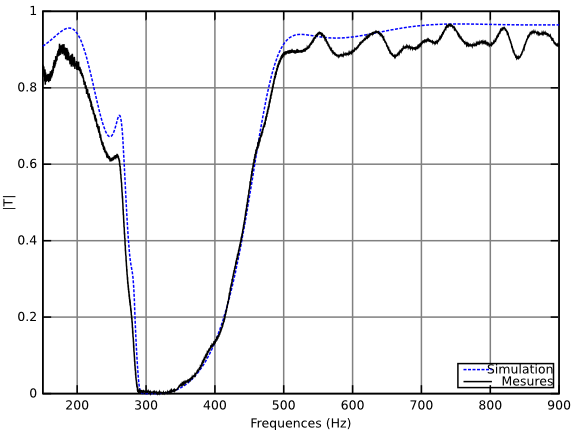
\includegraphics[scale=0.4]{images_chp3/5HR165_nodefect.png}\hfill
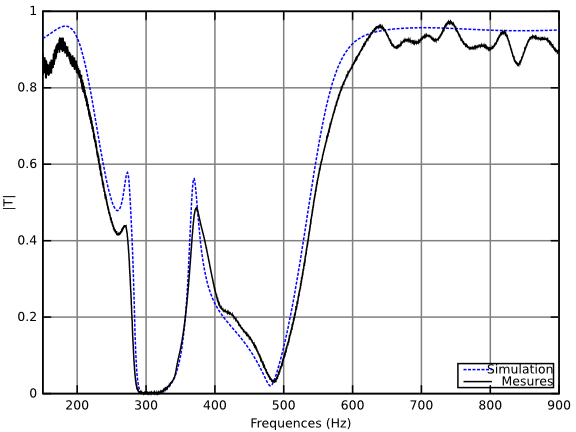
\includegraphics[scale=0.4]{images_chp3/5HR165_8cm_pos3.png}
\caption{\label{ref_trans1} Coefficients de transmission du réseau dans un cas sans défaut et avec défaut. Les courbes de simulations et de l’expérience sont superposées.}
\end{figure}

On constate qu'un pic de transmission est visible dans la bande interdite tant théoriquement qu'expérimentalement: le défaut permet à l'onde de traverser le réseau pour une fréquence donnée alors que dans le cas ou celui-ci n'est pas présent aucune transmission n'est possible. Ce comportement laisse supposer qu'un mode localisé est présent au niveau du défaut: si on augmente le nombre de résonateur, l'atténuation est plus forte et le pic disparaît, le mode est alors complètement localisé.

Ces résultats se retrouvent aussi sur la réflexion.
%
%\begin{figure}
%\centering
%\includegraphics[scale=0.3]{•}\hfill
%\includegraphics[scale=0.3]{•}
%\caption{\label{ref_trans1} Coefficient de transmission du réseau dans un cas sans défaut et avec défaut. Les courbes de simulations et de l'expériences sont superposées.}
%\end{figure}
\todo{coefficient de réflexion  pour ce truc la}

\section{Mesure d'un mode localisé par insertion de capteur dans le réseau}



Une fois la fréquence du mode de défaut relevée sur les coefficients de réflexions et transmissions on augmente le nombre de résonateurs de part et d'autre du défaut afin de créer un mode complètement localisé. Afin de pouvoir quand même exciter le mode localisé, une source est placé dans un des orifices au voisinage du défaut. Un microphone est inséré dans le réseau afin de mesure la pression en n'importe quel point. La pression RMS mesurée dans le tube est représenté figure ~\ref{p_tube} pour une configuration avec et sans défaut.

\begin{figure}[!h]
\centering
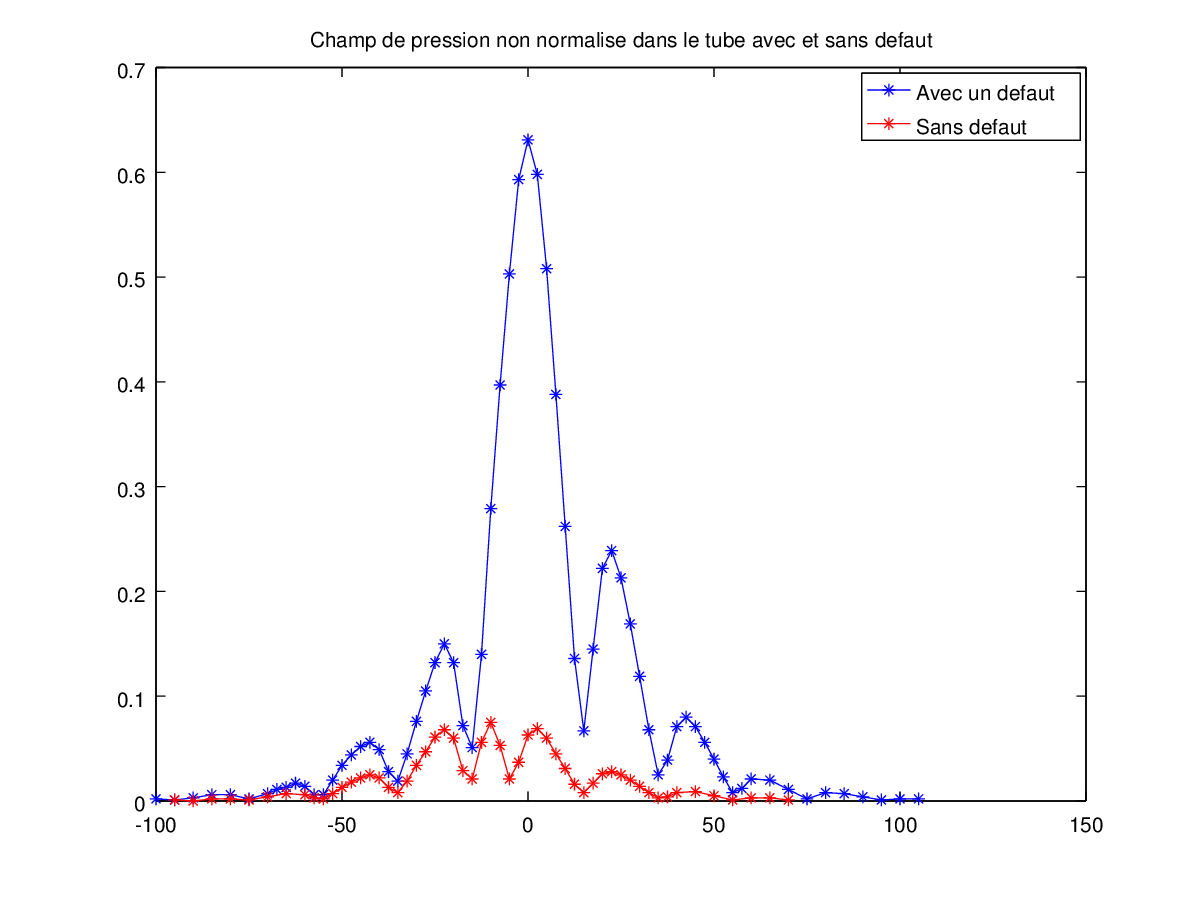
\includegraphics[scale=0.5]{./images_chp3/non_norm_lin.png}
\caption{\label{_tube} Pression RMS mesurée dans le réseau afin de mettre en évidence un mode localisé.}
\end{figure}

On constate que les niveaux de pression mesurés sont près de 10 fois plus élevé dans le cas ou un défaut est présent. De plus, la décroissance à mesure qu'on s'éloigne du défaut est très importante: on est donc bien en présence d'un mode localisé. Il est a noté que dans cette configuration le niveau maximum dans le réseau ne ce situe pas au niveau de la source mais du défaut (ce qui n'est pas le cas quand il n'y a pas de défaut).
\bigskip
Pour des questions matériels il n'a pas été possible de placer la source au même endroit que le défaut dans le réseau, la symétrie du système n'est donc pas conservée. C'est pourquoi les 2 courbes figurent \ref{p_tube} ne sont pas centré sur le même point. La courbe sans défaut est centrée sur la source et la courbe avec défaut est centré sur le défaut. 

\subsection{Changement de géométrie du défaut}
Afin de pouvoir étudier la différence de décroissance entre les 2 courbes, on change la géométrie du défaut: celui-ci est maintenant constitué de 2 résonateurs afin de pouvoir placer la source au centre. On à alors des cellule constitués de 2 résonateurs (voir schéma figure \ref{fig_exp}. La source se trouve en $x=0$, les résonateurs ont une longueur de cavité de $16~cm$ et ceux du défaut une longueur de $8~cm$. Ces longueurs sont modifiés par rapport au cas précédent car le mode localisé à lieu a une fréquence différente que dans le cas d'un défaut d'un seul résonateur: le couplage de 2 résonateur abaisse la fréquence du mode localisé (dans les fait 2 modes localisés sont créé, un plus basse fréquence et un plus haute, on choisi celui basse fréquence car il est mieux placé). On prend donc des cavités plus faible pour partir d'une plus haute fréquence.

\begin{figure}[!h]
\centering
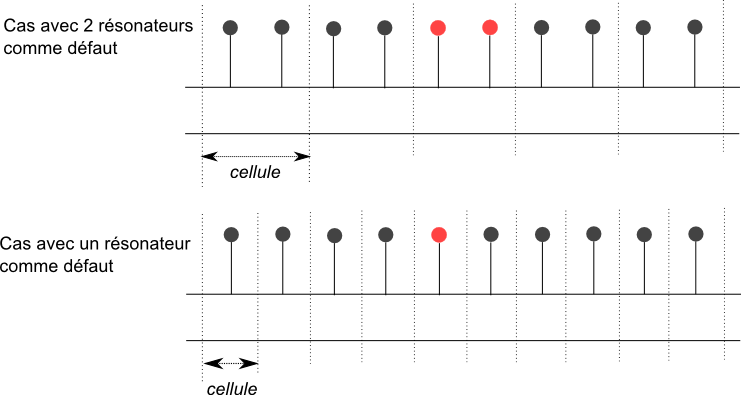
\includegraphics[scale=0.3]{./images_chp3/chgmt_defaut.png}
\caption{\label{fig_exp} Schéma décrivant le changement du défaut afin de rendre l'expérience symétrique.}
\end{figure}



On obtient les courbes de pression figure \ref{p_tube2}.

\begin{figure}[!h]
\centering
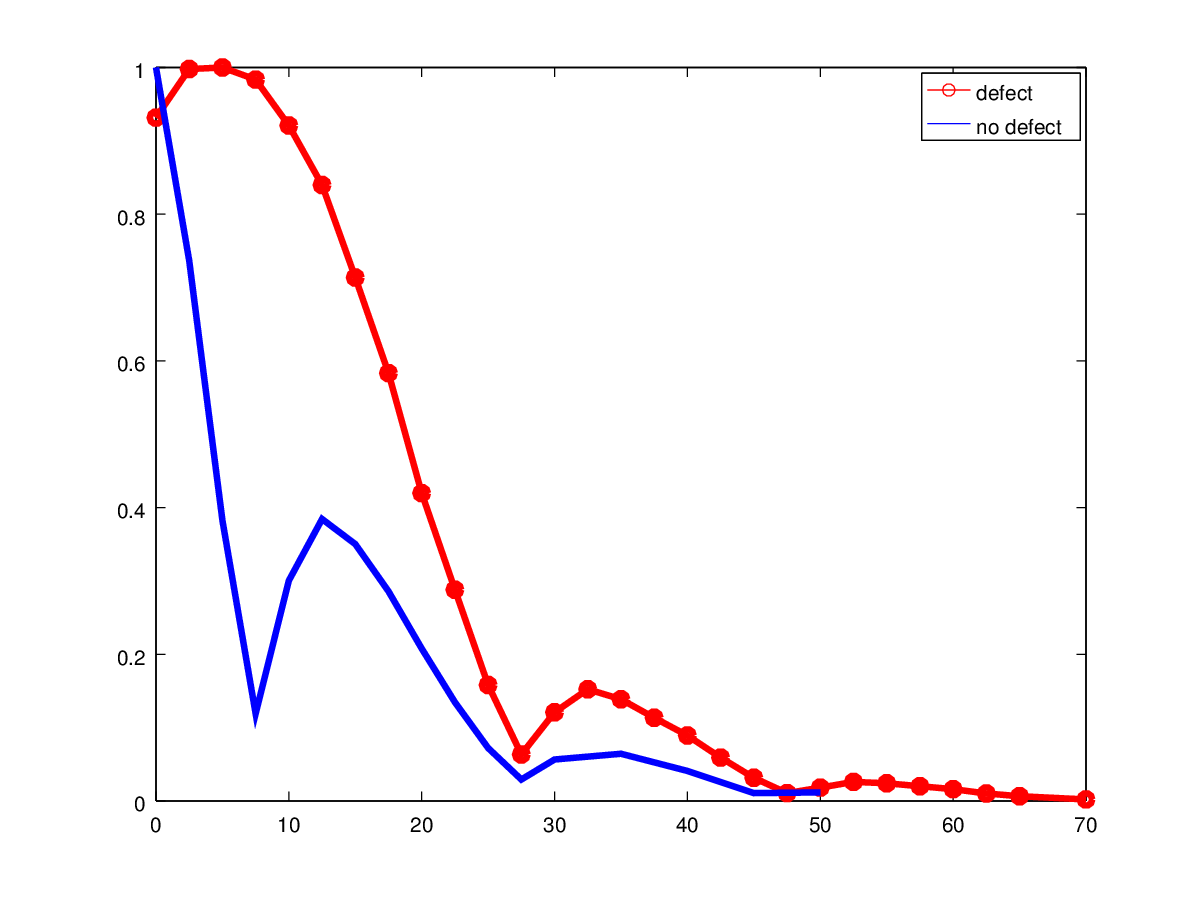
\includegraphics[scale=0.3]{./images_chp3/comparaison_decroissance_lin.png}\hfill
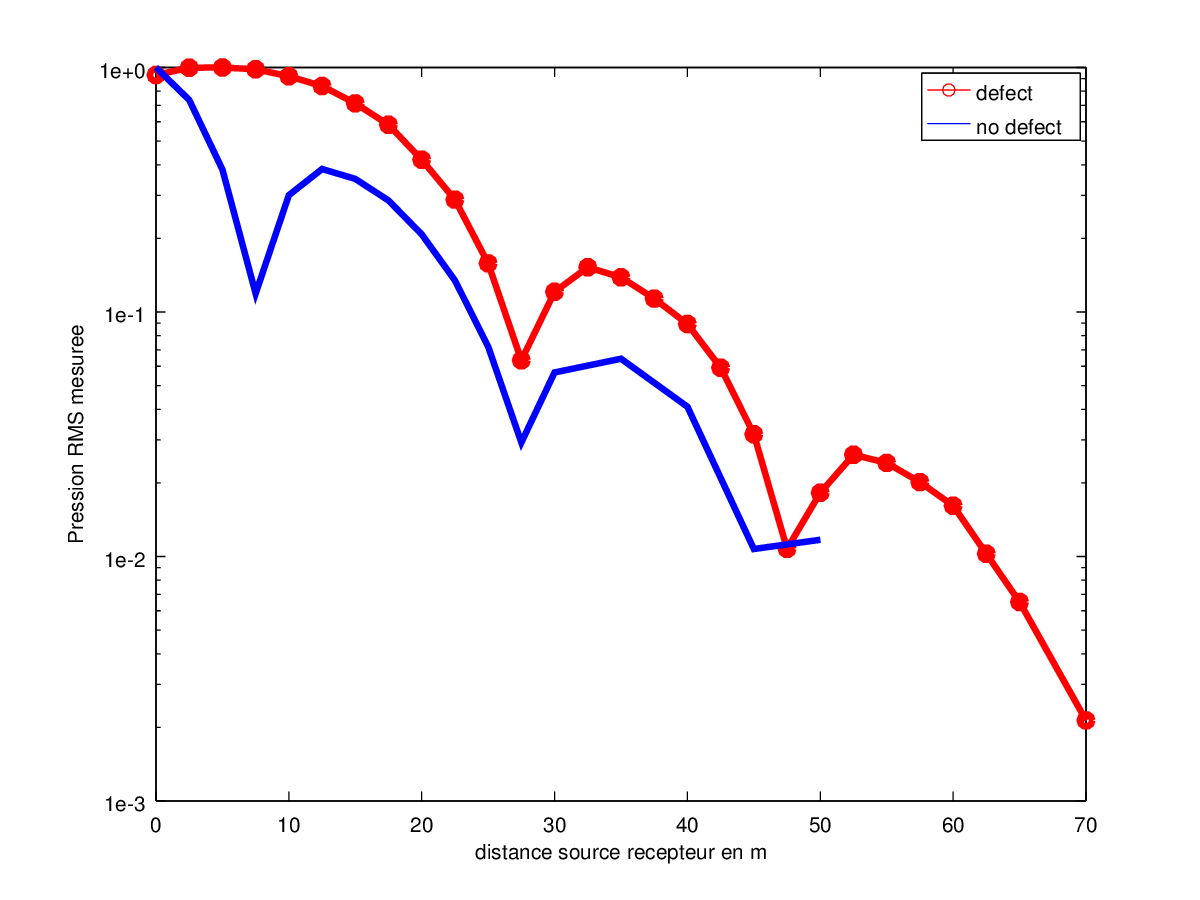
\includegraphics[scale=0.3]{./images_chp3/comparaison_decroissance_log.png}
\caption{\label{_tube} Pression RMS mesurée dans le réseau avec un défaut à 2 résonateurs. A gauche en abscisse linéaire, a droite en abscisse logarithmique.}
\end{figure}

Les décroissances semblent les mêmes pour les 2 courbes: le défaut à donc juste pour effet d'augmenter le niveau sonore mais n'induit pas une décroissance plus forte.


